%!TEX root = ../dokumentation.tex

\chapter{Parsen und Datenstruktur}
Der erste Schritt zum automatischen Beweisen eines Tableau, ist das Parsen der String-Repräsentation zu einer vom Programm weiterverarbeitbaren Datenstruktur. Hierfür wird im folgenden zuerst die Syntax definiert in der die Formeln als String dargestellt werden. Danach wird die Datenstruktur in der die Formel weiterverarbeitet wird besprochen. Zuletzt wird der Parser und die Implementierung dessen behandelt.

\section{Syntaxdefinition}
Prinzipiell wurde die Syntax in der die Formeln als String repräsentiert werden bereits in \autoref{sec:ind_form_regeln} beschrieben. Da die Buchstaben zur Darstellung der Junktoren aber auf handelsüblichen Tastaturen nicht vorhanden sind, müssen hierfür benutzerfreundlichere Alternativen definiert werden. Da die Zielgruppe des Tableaubeweisers meist schon mit Programmiersprachen in Berührung gekommen ist, wird sich dabei an den in Programmiersprachen üblichen Buchstaben orientiert. So wird z.B. für das Oder ($\vee$) das in Java, C\#, Swift und weiteren verwendete | definiert (in diesen Sprachen steht das einfache | für ein Bitweises-Oder, in diesem Fall gibt es allerdings keine Integer-Werte was eine Unterscheidung sinnlos macht).

Die vollständige Definition der insgesamt 7 Junktoren zu ihren Tastaturfreundlichen gegenspielern wird in \autoref{tbl:junktor_mapping} aufgeführt.
\begin{table}[h]
\begin{center}
\begin{tabular}{|c|c|c|c|}
\hline
Junktor-Symbol & Tastaturfreundliches Symbol & Alternatives Symbol \\
\hline
$\forall$ & (A) & /\textbackslash \\
\hline
$\exists$ & (E) & \textbackslash/ \\
\hline
$\neg$ & ! & - \\
\hline
$\wedge$ & \& & * \\
\hline
$\vee$ & | & + \\
\hline
$\rightarrow$ & -> & \\
\hline
$\leftrightarrow$ & <-> & \\
\hline
\end{tabular}
\end{center}
\caption{\label{tbl:junktor_mapping}Definition der tastaturfreundlichen Junktor-Symbole}
\end{table}

Zur Darstellung für Klammern werden nach wie vor die Runden Klammern ( und ) verwendet.

Ebenfalls zur Definition der Syntax gehört es zu definieren in welcher Form die atomaren Aussagen sowie Variablen, Konstanten und Funktionen in der Prädikatenlogik angegeben werden. Da es in der klassischen sowie nichtklassischen Aussagenlogik kein Risiko für Ambiguitäten zwischen Funktion und Prädikat oder ähnlichem gibt, dürfen diese mit Klein- und Großbuchstaben beginnen. Zudem darf die atomare Aussage Zahlen und Unterstriche enthalten, muss aber mit einem Buchstaben beginnen.

Bei der klassischen und nichtklassischen Prädikatenlogik kann es allerdings zu besagten Ambiguitäten kommen. Um bereits an der Schreibweise zu klären um was es sich handelt werden hier folgende Regeln eingeführt:
\begin{itemize}
\item \textbf{Prädikat}: Ein Prädikat muss mit einem Großbuchstaben beginnen. Danach kann dieses beliebe Klein- und Großbuchstaben sowie Zahlen und Unterstriche enthalten.

\item \textbf{Funktion}: Ein Prädikat muss mit einem Kleinbuchstaben beginnen. Danach kann dieses beliebe Klein- und Großbuchstaben sowie Zahlen und Unterstriche enthalten.

\item \textbf{Konstante}: Eine Konstante muss mit einem Großbuchstaben beginnen. Danach kann dieses beliebe Klein- und Großbuchstaben sowie Zahlen enthalten.

\item \textbf{Variable}: Eine Variable muss mit einem Kleinbuchstaben beginnen. Danach kann dieses beliebe Klein- und Großbuchstaben sowie Zahlen enthalten.
\end{itemize}

Man beachte, dass Konstanten und Variablen keine Unterstriche enthalten dürfen. Dies liegt daran, dass während des automatischen Beweisens von Prädikatenlogischen Aussagen unter Umständen neue Konstanten eingeführt werden. Um keine Analyse der existierenden Konstanten durchführen zu müssen um zu berechnen welche Konstanten noch nicht eingeführt sind, wird das Unterstrich-Zeichen für diese Konstanten reserviert. Eine dadurch eingeführte Konstante wird dann als ``X\_n'' eingeführt wobei n der Index der eingeführten Konstante ist.


\section{Datenstruktur}
Mit einer Formel in der oben definierten Syntax kann nicht direkt weitergearbeitet werden. Um dies zu tun, muss diese in einer Datenstruktur vorliegen, mit der ein Computer sinnvoll rechnen kann.
Deshalb wird diese in einen Syntaxbaum geparsed. In einem Syntaxbaum stellt jeder innere Knoten einen Operator und jeder Kind-Knoten einen Operanden der Operatoren. \cite{compiler_dragon_book} In diesem Fall wären die Kind-Knoten die atomaren Aussagen. Ein Beispiel eines solchen Syntaxbaums für die Aussage A$\vee$B$\rightarrow\neg$C ist in \autoref{fig:example_syntax_tree} dargestellt.

\begin{figure}[H]
\begin{center}
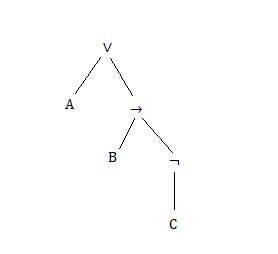
\includegraphics[scale=1]{images/example_syntax_tree.png}
\caption{Beispiel eines Syntaxbaumes der Aussage A$\vee$B$\rightarrow\neg$C}
\label{fig:example_syntax_tree}
\end{center}
\end{figure}

Das Konzept eines Syntaxbaums übersetzt in die für diese Arbeit verwendete objektorientierte Programmiersprache Python, ergibt eine Datenstruktur in der die einzelnen Operatoren und atomaren Aussagen Objekten entsprechen die jeweils ihre Kind-Knoten als variablen halten. Das Klassendiagramm für die Aussagenlogik ist in \autoref{fig:class_diag_ds_pl} zu sehen.

\begin{figure}[H]
\begin{center}
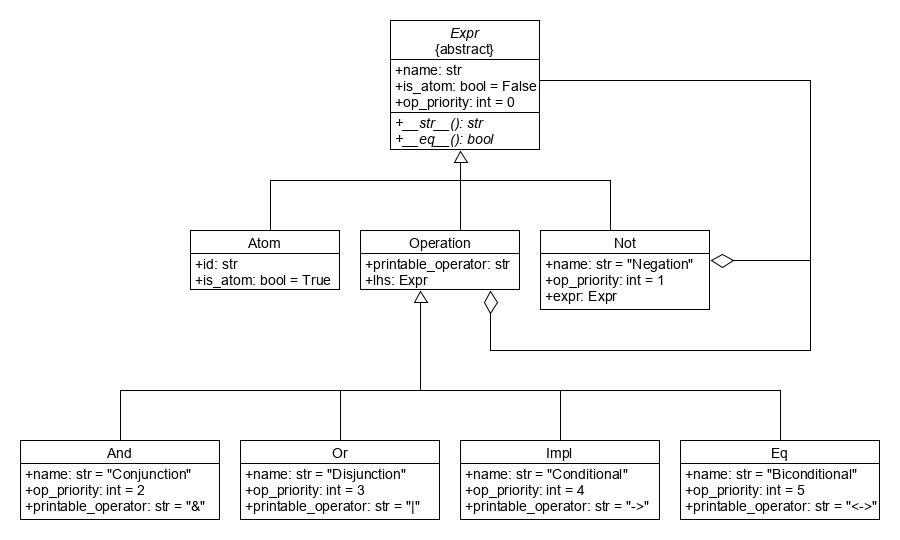
\includegraphics[scale=0.5]{images/class_diag_ds_pl.png}
\caption{Klassendiagramm der Aussagenlogik}
\label{fig:class_diag_ds_pl}
\end{center}
\end{figure}

Der Syntaxbaum für die Prädikatenlogik sieht mehr oder weniger ähnlich aus. Der große Unterschied hierbei ist die atomare Aussage. Diese ist in der Prädikatenlogik die Klasse \textit{Predicate} wobei diese eine Liste von Termen, also Funktionen, Konstanten und Variablen hält. Zudem gibt es die beiden weiteren Quantifikatoren-Klassen. Der Ausschnitt aus dem Klassendiagramm mit den zusätzlichen Klassen ist in \autoref{fig:class_diag_ds_fopl} dargestellt.

\begin{figure}[H]
\begin{center}
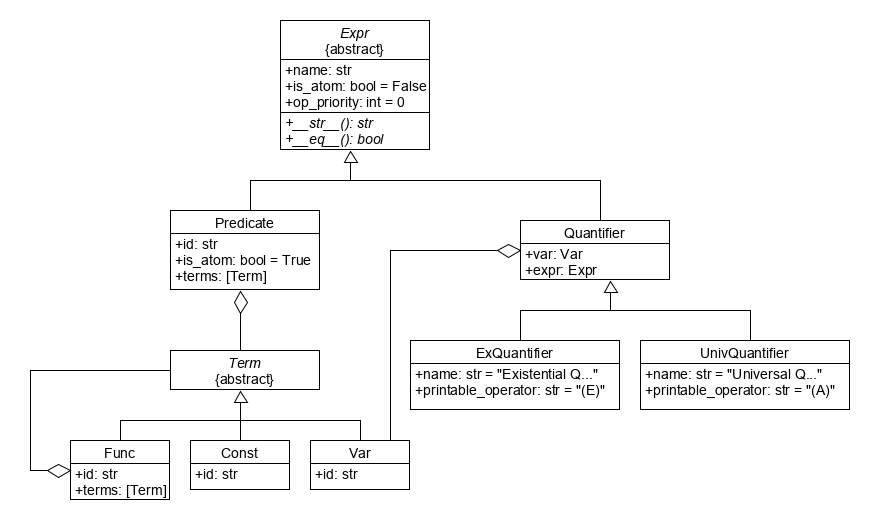
\includegraphics[scale=0.5]{images/class_diag_ds_fopl.png}
\caption{Ausschnitt des Klassendiagramm der Prädikatenlogik}
\label{fig:class_diag_ds_fopl}
\end{center}
\end{figure}

In der definierten Datenstruktur sieht der in \autoref{fig:example_syntax_tree} dargestellte Syntaxbaum also wie im Objektdiagramm in \autoref{fig:obj_diag_syn_tree} zu sehen aus.

\begin{figure}[H]
\begin{center}
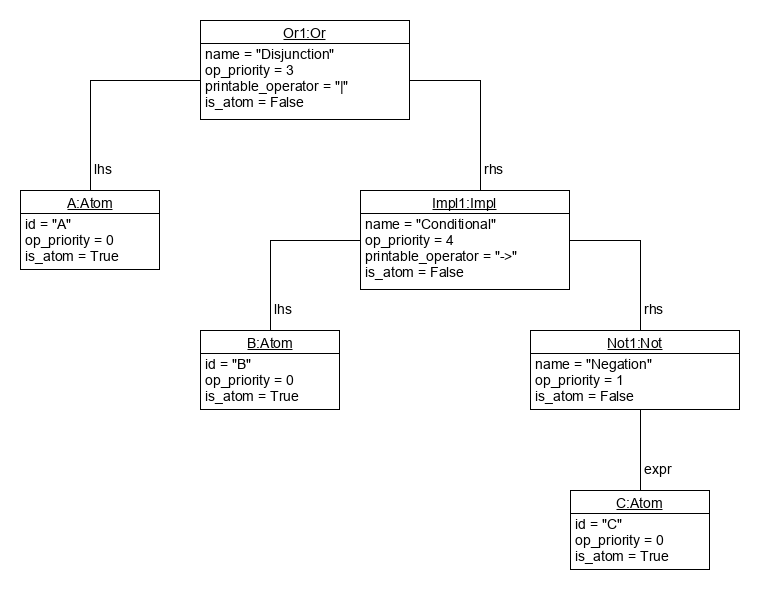
\includegraphics[scale=0.5]{images/obj_diag_syn_tree.png}
\caption{Objektdiagramm des Syntaxbaums der Aussage A$\vee$B$\rightarrow\neg$C}
\label{fig:obj_diag_syn_tree}
\end{center}
\end{figure}


\section{Parsen}
Da nun klar ist, wie die Syntax und Datenstruktur der Formeln aussieht, muss noch die Zeichenketten-Repräsentation zur Datenstruktur geparsed werden.

Zum erstellen des Parsers, wird der Parsergenerator ANTLR verwendet. Mit ANTLR kann eine Grammatik definiert werden von der dann ein LL(*)-Parser in einer von vielen möglichen Programmiersprachen generiert wird. Generiert werden kann unter anderem Java, C\#, JavaScript aber auch Python. \cite{antlr_doc}

\subsection{LL(*)-Parser}
Der vorherrschende Parsertyp beruht auf einer LR(k)-Syntaxanalyse, wobei das ``L'' für das Durchgehen der Eingabe von links nach rechts steht, das ``R'' für das Erstellen der umgekehrten Rechtsableitung und das k dafür, wie viele Eingabesymbole bei Entscheidungen während der Analyse im Voraus betrachtet werden. \cite{compiler_dragon_book}

Diese Methode wird von den durch ANTLR generierten Parsern allerdings nicht angewandt. Für von ANTLR generierte Parser, wird ein eigens für ANTLR entwickeltes Verfahren Namens LL(*) verwendet. \cite{ll_star_parser}







